\newpage
\section{Mandelbrot Set}

\subsection{Definition}
The Mandelbrot fractal is defined as a set of points in the complex plane.  
Each point corresponds to a complex number \( c \).\\

\noindent
For every \( c \), we consider the iterative sequence:
\[
z_0 = 0, \qquad z_{n+1} = z_n^2 + c
\]

\noindent
We then observe the behavior of \( z_n \) as \( n \to \infty \).\\

\subsubsection{Point that belongs to the Mandelbrot set}
Take \( c = -1 \). Then the sequence is
\[
z_0 = 0, \quad 
z_1 = 0^2 + (-1) = -1, \quad
z_2 = (-1)^2 + (-1) = 0, \quad
z_3 = 0^2 + (-1) = -1, \dots
\]
\noindent
The results remain bounded, so \( c = -1 \) belongs to the Mandelbrot set.

\subsubsection{Point that does NOT belong to the Mandelbrot set}
Take \( c = 1 \). Then the sequence is
\[
z_0 = 0, \quad
z_1 = 0^2 + 1 = 1, \quad
z_2 = 1^2 + 1 = 2, \quad
z_3 = 2^2 + 1 = 5, \dots
\]  
\noindent
The values grow up to infinite, so \( c = 1 \) does not belong to the Mandelbrot set.\\

\subsection{Images}
This process gives rise to the famously intricate structure of the Mandelbrot fractal. Here a simple explanation \cite{simple} or here a more complex one \cite{formal} and here an online demo \cite{demo}.\\

\begin{figure}[h!]
    \centering
    
\includegraphics[width=0.23\linewidth]{assets/mandelbrot/Mandel_zoom_00_mandelbrot_set.jpg} \hfill
    
\includegraphics[width=0.23\linewidth]{assets/mandelbrot/Mandel_zoom_01_head_and_shoulder.jpg} \hfill
    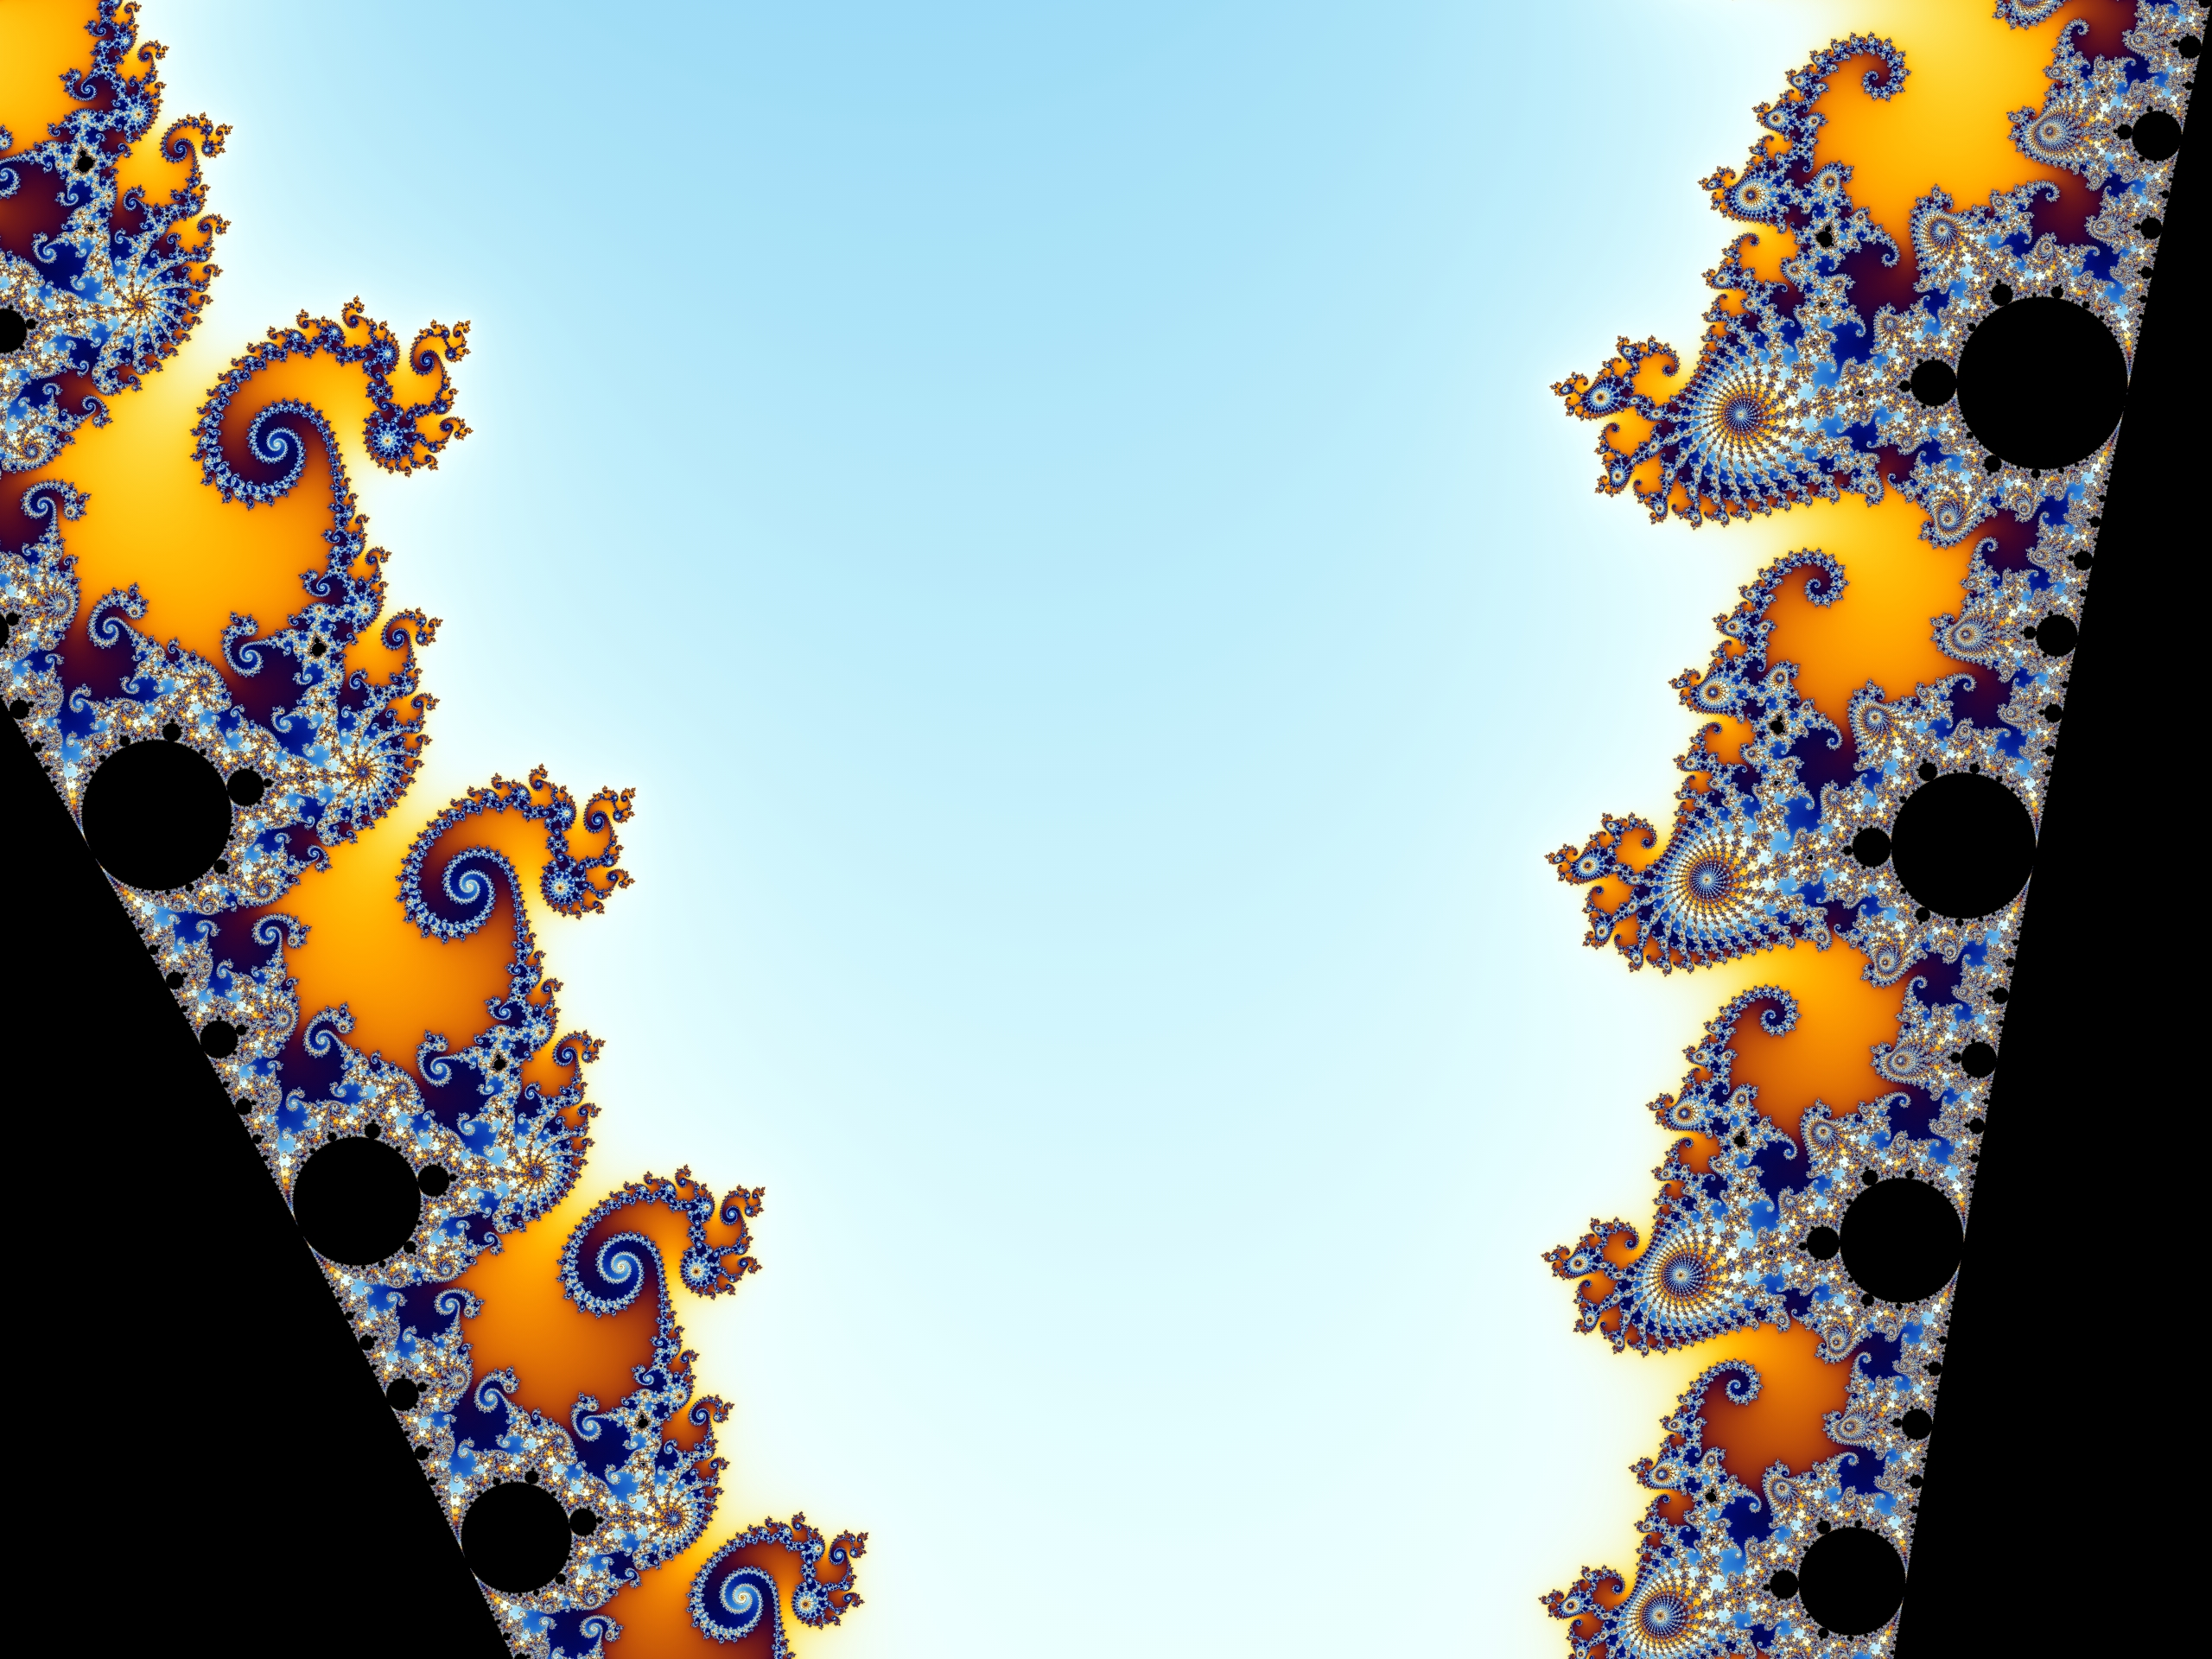
\includegraphics[width=0.23\linewidth]{assets/mandelbrot/Mandel_zoom_02_seehorse_valley.jpg} \hfill
    
\includegraphics[width=0.23\linewidth]{assets/mandelbrot/Mandel_zoom_03_seehorse.jpg}
\end{figure}

\noindent
The color represents how quickly the values of \( z_n \) grow:  
\begin{itemize}
    \item[] \textbf{Black} - the sequence remains bounded;
    \item[] \textbf{Other colors} - the sequence escapes to infinity, with the color indicating how fast it diverges.  
\end{itemize}